\newpage
\onecolumn
\appendix
\section*{{\huge Appendix}}
\label{sec:appendix}

\section{Sinkhorn Algorithm}

Given $\boldsymbol{\alpha}$, $\boldsymbol{\beta}$ and $\boldsymbol{D}$, the OT distance between empirical probability measures $f$ and $g$ is a linear programing problem:
\begin{equation}
    d_{W}(\boldsymbol{\alpha},\boldsymbol{\beta},\boldsymbol{D}) = \min_{\boldsymbol{T} \in U(\boldsymbol{\alpha},\boldsymbol{\beta})} \langle \boldsymbol{T},\boldsymbol{D} \rangle.
\end{equation}

The solution to obtain the optimal transport plan $\boldsymbol{T}$ is quite computationally expensive. Cuturi \citep{distances2013lightspeed}
introduced an entropy constraint to the transportation polytope, converting the original problem to an entropy regularized optimal transportation problem, resulting in \textit{Sinkhorn distance}, i.e:
\begin{equation}\label{eq5}
\begin{aligned}
    d_{S}^\lambda (\boldsymbol{\alpha}, \boldsymbol{\beta}, \boldsymbol{D}) = \langle \boldsymbol{T}^\lambda, \boldsymbol{D} \rangle 
    \\
    \text{s.t.} \quad \boldsymbol{T}^\lambda = \argmin_{\boldsymbol{T} \in U(\boldsymbol{\alpha}, \boldsymbol{\beta)}} \langle \boldsymbol{T}, \boldsymbol{D} \rangle - \frac{1}{\lambda} h(\boldsymbol{T}),
\end{aligned}
\end{equation}
where $h(\boldsymbol{T}) = - \sum_{i=1}^N \sum_{j=1}^M t_{ij}\log t_{ij}$ is the entropy of $\boldsymbol{T}$. The optimal $\boldsymbol{T}^\lambda$ that minimizes (\ref{eq5}) is:
\begin{equation}
    \label{eq:solution}
    \boldsymbol{T}^\lambda = diag(\boldsymbol{\kappa}_1) \exp^{-\lambda\boldsymbol{D}} diag(\boldsymbol{\kappa}_2)
\end{equation}
where $\exp^{-\lambda\boldsymbol{D}}$ is the element-wise exponential of the matrix $-\lambda\boldsymbol{D}$, $\boldsymbol{\kappa}_1 \in \mathbb{R}^N$, $\boldsymbol{\kappa}_2 \in \mathbb{R}^M$ are the non-negative scaling factors, which can be effectively solved after some Sinkhorn iterations. Hence, the computational cost is greatly reduced compare with the original problem.

\section{Experimental Details}

\paragraph{Models.} We select GPT2-120M \cite{radford2019language},TinyLLaMa-1.1B \cite{zhang2024tinyllama} and GPT2-1.5B as student LLMs. For teachers, we employ GPT2-1.5B, Qwen1.5-1.8B \cite{bai2023qwen}, LLaMa2-7B \cite{touvron2023llama}, Mistral-7B \cite{jiang2023mistral} and Qwen2.5-7B-Instruct \cite{yang2024qwen2}
as teacher LLMs for same and different vocabularies settings. The detail of each models training configurations in KD is listed in Table \ref{tab:kd_configurations}.

\begin{table*}[!ht]
\centering
\begin{adjustbox}{width=0.8\textwidth}
\begin{tabular}{lccc cc ccc}
\toprule
\textbf{Settings} 
    & \multicolumn{3}{c}{\textbf{KD for GPT2-base}} 
    & \multicolumn{2}{c}{\textbf{KD for GPT2}} 
    & \multicolumn{3}{c}{\textbf{KD for TinyLLama}} \\
\cmidrule(lr){2-4} \cmidrule(lr){5-6} \cmidrule(lr){7-9}
    & \textbf{GPT2-base} & \textbf{Qwen1.5} & \textbf{GPT2-large} 
    & \textbf{GPT2-large} & \textbf{Qwen2.5} 
    & \textbf{TinyLLama} & \textbf{LLaMA2} & \textbf{Mistral} \\
\midrule
\textbf{Epoch} 
    & 20 & 10 & 20 
    & 10 & 10 
    & 10 & 10 & 10 \\
\textbf{LR} 
    & $5\times10^{-4}$ & $2\times10^{-5}$ & $5\times10^{-4}$ 
    & $2\times10^{-5}$ & $1\times10^{-3}$ 
    & $1\times10^{-3}$ & $1\times10^{-3}$ & $1\times10^{-3}$ \\
\textbf{Projector LR} 
    & $1\times10^{-3}$ & $1\times10^{-3}$ & $1\times10^{-3}$ 
    & $1\times10^{-3}$ & $1\times10^{-3}$ 
    & $1\times10^{-3}$ & $1\times10^{-3}$ & $1\times10^{-3}$ \\
\textbf{Batch Size} 
    & 32 & 32 & 32 
    & 32 & 32 
    & 32 & 32 & 32 \\
\textbf{LR Scheduler} 
    & Cosine & Cosine & Cosine 
    & Cosine & Cosine 
    & Cosine & Cosine & Cosine \\
\textbf{Fine-Tuning Method} 
    & Full & Full & Full 
    & Full & LoRA 
    & LoRA & LoRA & LoRA \\
\textbf{LoRA Rank} 
    & N/A & N/A & N/A 
    & 256 & 256 
    & 256 & 256 & 256 \\
\textbf{LoRA Alpha} 
    & N/A & N/A & N/A 
    & 8 & 8 
    & 8 & 8 & 8 \\
\textbf{LoRA Dropout} 
    & N/A & N/A & N/A 
    & 0.1 & 0.1 
    & 0.1 & 0.1 & 0.1 \\
\bottomrule
\end{tabular}
\end{adjustbox}
\caption{Detailed training configurations}
\label{tab:kd_configurations}
\end{table*}

\paragraph{Training and Evaluation.}
For GPT2-120M, we employ full fine-tuning for students and teachers, while for TinyLLaMa and GPT2-large we fine-tune the students and teacher with LoRA \cite{hu2021lora}. For evaluation, we sample the responses of models from 5 random seeds. The performance is evaluated by \textbf{ROUGE-L} \cite{lin2004rouge}, a measure of similarity between the generated response and the ground truth. All the experiments are conducted on 4 A100 80GB GPUs.

\paragraph{Detailed Dataset Statistics.} Table \ref{tab:dataset} provides statistics on the number of samples in the training, validation, and test sets for each domain-specific dataset.

% \paragraph{Hyperparameter.} Table \ref{tab:alpha_params} provides detailed hyperparameter $\alpha$ values for each setting.
\paragraph{Hyperparameter.} 

We searched for the hyperaparameter $\alpha$ within the range \(\{0.1, 0.5, 0.6, 0.9\}\) and the best value for each experimental scenario is reported as in Table~\ref{tab:alpha_params}.


% \paragraph{} Table \ref{tab:dataset} provides statistics on the number of samples in the training, validation, and test sets for each domain-specific dataset.

\begin{table}[ht]
\centering
\begin{adjustbox}{width=0.35\textwidth}
\begin{tabular}{l|c|c|c}
\toprule
Dataset   & Train & Validation & Test \\ \midrule
\textbf{Dolly}   & 11435 & 1000 & 500 \\
\textbf{Alpaca}   & 10396 & 500 & 500 \\
\textbf{S-NI}   & 10414 & 500 & 1902 \\
\textbf{DialogSum}   & 12460 & 500 & 1500\\ 
\bottomrule

\end{tabular}
\end{adjustbox}
\caption{Dataset Statistics}
\label{tab:dataset}
\end{table}



\begin{table*}[ht]
\scriptsize
\centering
\begin{adjustbox}{width=0.7\textwidth}
\begin{tabular}{l|c|c|c|c}
\toprule
\textbf{Methods} & \textbf{Dolly} & \textbf{Alpaca} & \textbf{S-NI} & \textbf{Dialogue Sum} \\
\midrule
\multicolumn{5}{l}{\textit{\textbf{Student: GPT2-120M}}} \\
\hline
\multicolumn{5}{c}{\textit{Teacher: GPT2-1.5B (Same Vocabulary)}} \\
\hline
KL + \method & $0.6$ & $0.5$ & $0.5$ & $0.5$ \\
\hline  
\multicolumn{5}{c}{\textit{Teacher: Qwen1.5-1.8B (Different Vocabularies)}} \\
\hline
ULD + \method  & $0.5$ & $0.5$ & $0.5$ & $0.5$ \\
MinED + \method & $0.5$ & $0.5$ & $0.5$ & $0.5$ \\
DSKD + \method  & $0.1$ & $0.9$ & $0.9$ & $0.9$ \\
\bottomrule
\toprule
\multicolumn{5}{l}{\textit{\textbf{Student: TinyLLaMA-1.1B}}} \\
\hline
\multicolumn{5}{c}{\textit{Teacher: Llama2-7B (Same Vocabulary)}} \\
\hline 
KL + \method & $0.6$ & $0.6$ & $0.5$ & $0.5$ \\
\hline
\multicolumn{5}{c}{\textit{Teacher: Mistral-7B (Different Vocabularies)}} \\
\hline 
ULD + \method  & $0.5$ & $0.5$ & $0.6$ & $0.5$ \\
MinED + \method & $0.5$ & $0.9$ & $0.5$ & $0.5$ \\
DSKD + \method  & $0.9$ & $0.9$ & $0.9$ & $0.9$ \\
\bottomrule   
\toprule 
\multicolumn{5}{l}{\textit{\textbf{Student: GPT2-1.5B}}} \\
\hline 
\multicolumn{5}{c}{\textit{Teacher: Qwen2.5-7B-Instruct (Different Vocabularies)}} \\
\hline
ULD + \method  & $0.5$ & $0.5$ & $0.5$ & $0.5$ \\
MinED + \method & $0.5$ & $0.5$ & $0.5$ & $0.9$ \\
DSKD + \method   & $0.9$ & $0.9$ & $0.9$ & $0.9$ \\
\bottomrule
\end{tabular}
\end{adjustbox}
\caption{The best-searched hyperparameters $\alpha$ for different configurations}
\label{tab:alpha_params}
\end{table*}





\label{sec:appendix_exp}

\section{Prompts Details}

\begin{figure*}[ht]
\centering
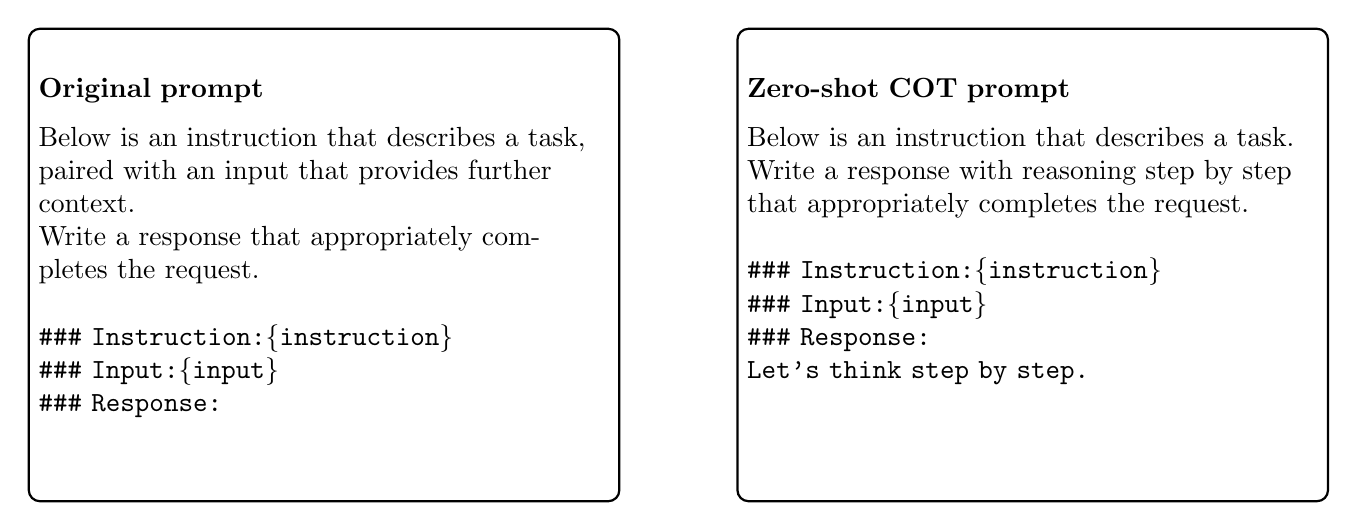
\begin{tikzpicture}
% Box for Original Prompt
\draw[rounded corners, thick] (0,0) rectangle (7.5,-6);
\node[anchor=north west, text width=7cm] at (0,-0.5) {
\textbf{Original prompt}
\vspace{0.2cm}

Below is an instruction that describes a task, paired with an input that provides further context.\\ 
Write a response that appropriately completes the request.

\texttt{\\\#\#\# Instruction:\{instruction\}\\\#\#\# Input:\{input\}\\\#\#\# Response:}
};

% Box for Zero-shot COT Prompt
\draw[rounded corners, thick] (9,0) rectangle (16.5,-6);
\node[anchor=north west, text width=7cm] at (9,-0.5) {
\textbf{Zero-shot COT prompt}
\vspace{0.2cm}

Below is an instruction that describes a task.\\ 
Write a response with reasoning step by step that appropriately completes the request.

\texttt{\\\#\#\# Instruction:\{instruction\}\\\#\#\# Input:\{input\}\\\#\#\# Response:\\ Let's think step by step.}
};
\end{tikzpicture}
\caption{Original Prompt and Zero-shot COT Prompt}
\label{fig:prompts}
\end{figure*}

\label{sec:prompt}


% \begin{table*}[ht]
% \centering
% \begin{adjustbox}{width=\textwidth}
% \begin{tabular}{l|ccc|cc|ccc}
% \toprule
% \parbox[c][2.5em][c]{1.5cm}{\centering \textbf{Settings}}
%     & \multicolumn{3}{c|}{\textbf{KD for GPT2-base}}
%     & \multicolumn{2}{c|}{\textbf{KD for GPT2}}
%     & \multicolumn{3}{c}{\textbf{KD for TinyLLama}} \\
% \cmidrule{2-9}
% & \textbf{GPT2-base} & \textbf{Qwen1.5} & \textbf{GPT2-large}
% & \textbf{GPT2-large} & \textbf{Qwen2.5}
% & \textbf{TinyLLama} & \textbf{LLaMA2} & \textbf{Mistral} \\
% \midrule
% \textbf{Epoch}
%     & 20 & 10 & 20 
%     & 10 & 10
%     & 10 & 10 & 10 \\
% \textbf{LR}
%     & 5e-4 & 2e-5 & 5e-4
%     & 2e-5 & 1e-3
%     & 1e-3 & 1e-3 & 1e-3 \\
% \textbf{Projector LR}
%     & 1e-3 & 1e-3 & 1e-3
%     & 1e-3 & 1e-3
%     & 1e-3 & 1e-3 & 1e-3 \\
% \textbf{Batch Size}
%     & 32 & 32 & 32
%     & 32 & 32
%     & 32 & 32 & 32 \\
% \textbf{LR Scheduler}
%     & Cosine & Cosine & Cosine
%     & Cosine & Cosine
%     & Cosine & Cosine & Cosine \\
% \textbf{Fine-Tuning Method}
%     & Full & Full & Full
%     & Full & LoRA
%     & LoRA & LoRA & LoRA \\
% \textbf{LoRA Rank}
%     & N/A & N/A & N/A
%     & 256 & 256
%     & 256 & 256 & 256 \\
% \textbf{LoRA Alpha}
%     & N/A & N/A & N/A
%     & 8 & 8
%     & 8 & 8 & 8 \\
% \textbf{LoRA Dropout}
%     & N/A & N/A & N/A
%     & 0.1 & 0.1
%     & 0.1 & 0.1 & 0.1 \\
% \bottomrule
% \end{tabular}%
% \end{adjustbox}
% \caption{Detailed training configurations}
% \label{tab:kd_configurations}
% \end{table*}
